\section{Schematy różnicowe dla zadań dyfuzyjnych}

Będziemy korzystać z równania:

\[
\begin{cases}
\vspace{0.1cm} 
\hspace{0,1cm} \dfrac{\delta \psi}{\delta t} = D\dfrac{\delta^2 \psi}{\delta x^2} \hspace{1cm}, \Omega = [0,L]x[0,\infty] \\
\vspace{0.1cm}
\hspace{0,1cm}\psi_{(x,t)}|_{x=0} = 0 \hspace{0.8cm},t>0 \\
\vspace{0.1cm} 
\hspace{0,1cm}\psi_{(x,t)}|_{x=L} = 0 \hspace{0.7cm},t>0 \\
\vspace{0.1cm} 
\hspace{0,1cm}\psi_{(x,t)}|_{t=0} = \varphi(x) \hspace{0.3cm},x\in[0,L]
\end{cases}
\]

\subsection{Cel ćwiczenia}

Naszym zadaniem było stworzenie algorytmu rozwiązującego następujące równanie:

\[
\begin{cases}
\vspace{0.1cm} 
\hspace{0,1cm} \dfrac{\delta \psi}{\delta t} = D\dfrac{\delta^2 \psi}{\delta x^2} \\
\vspace{0.1cm}
\hspace{0,1cm}\psi|_{x=0} = 0 \\
\vspace{0.1cm} 
\hspace{0,1cm}\psi|_{x=L} = 0 \\
\vspace{0.1cm} 
\hspace{0,1cm}\psi|_{t=0} = sin(\frac{\pi x}{2})
\end{cases}
\]

, gdzie:

$\Omega = [0,2]x[0,1]$
\newline
$D=1$
\newline
\vspace{0.2cm}
$\psi_{analityczna}=\psi(x,t)=sin\Big(\dfrac{\pi x}{2}\Big)e^{-\Big(\dfrac{\pi^2 t}{4}\Big)}$

\subsection{Schemat FTCS}

FTCS (ang. Forward Time Central Space) czyli schemat "w przód":

$$\dfrac{\delta \psi}{\delta t} = D\dfrac{\delta^2 \psi}{\delta x^2}$$

Dla lewej strony równania zastosujemy schemat "w przód", natomiast dla prawej schemat centralny.

Mamy więc:

$$\dfrac{\psi^{(n+1)}_{i}-\psi^n_{i}}{\Delta t}=D\dfrac{\psi^{n}_{i+1}-2\psi^n_{i}+\psi^n_{i-1}}{\Delta x^2}$$

Stąd:

$$\psi^{(n+1)}_{i}=\dfrac{D\Delta t}{\Delta x^2}\Big(\psi^{n}_{i+1}-2\psi^{n}_{i}+\psi^{n}_{i-1}\Big)+\psi^{n}_{i} + O(\Delta t)+O(\Delta x^2)$$

Jest to schemat jawny, warunkowo stabilny, a więc parametry siatki muszą zostać dobrane we właściwy sposób.

Warunkiem stabilności dla takiego zadania jest następująca relcja:

$$\dfrac{D\Delta t}{\Delta x^2}\le \dfrac{1}{2}$$
\newpage
\subsubsection{Algorytm}

\begin{Shaded}
\begin{Highlighting}[]
\FunctionTok{clc}\NormalTok{,}\FunctionTok{clear} \FunctionTok{all}
\FunctionTok{tic}
\CommentTok{%rozwiązanie analityczne}
\NormalTok{G = @(x,t) }\FunctionTok{sin}\NormalTok{(}\BaseNTok{pi}\NormalTok{.*x./}\FloatTok{2}\NormalTok{).*}\FunctionTok{exp}\NormalTok{(-(}\BaseNTok{pi}\NormalTok{.^}\FloatTok{2}\NormalTok{).*t./}\FloatTok{4}\NormalTok{);}

\CommentTok{%przedział omega}
\NormalTok{xa=}\FloatTok{0}\NormalTok{;}
\NormalTok{xb=}\FloatTok{2}\NormalTok{;}
\NormalTok{yc=}\FloatTok{0}\NormalTok{;}
\NormalTok{yd=}\FloatTok{1}\NormalTok{;}

\CommentTok{%warunki brzegowe}
\NormalTok{u1 = @(x) }\FloatTok{0}\NormalTok{;}
\NormalTok{u2 = @(x) }\FloatTok{0}\NormalTok{;}
\NormalTok{u3 = @(x,t) }\FunctionTok{sin}\NormalTok{(}\BaseNTok{pi}\NormalTok{*x/}\FloatTok{2}\NormalTok{);}

\NormalTok{licznik=}\FloatTok{0}\NormalTok{;}
\CommentTok{%siatka}
\NormalTok{m=}\FloatTok{30}\NormalTok{;}
\NormalTok{D=}\FloatTok{1}\NormalTok{;}
\NormalTok{deltax=(xb-xa)/(m-}\FloatTok{1}\NormalTok{);}
\NormalTok{x=[xa:deltax:xb];         }\CommentTok{%przedział przestrzenny}
\NormalTok{deltat=(deltax^}\FloatTok{2}\NormalTok{)/(}\FloatTok{20}\NormalTok{*D); }\CommentTok{%dzielimy od razu przez 10, aby wartość }
\NormalTok{n_end=}\FunctionTok{floor}\NormalTok{(yd/deltat)+}\FloatTok{1}\NormalTok{; }\CommentTok{%nie była blisko deltat graniczne}
\NormalTok{t=[}\FloatTok{0}\NormalTok{:deltat:}\FloatTok{1}\NormalTok{];           }\CommentTok{%przedział czasowy}

\CommentTok{%macierz}
\FunctionTok{psi}\NormalTok{=}\FunctionTok{zeros}\NormalTok{(n_end,}\FunctionTok{length}\NormalTok{(x)); }\CommentTok{%utworzenie pustej macierzy}

\NormalTok{for }\BaseNTok{i}\NormalTok{=}\FloatTok{2}\NormalTok{:m-}\FloatTok{1}                \CommentTok{%dodanie warunku początkowego}
  \FunctionTok{psi}\NormalTok{(}\FloatTok{1}\NormalTok{,}\BaseNTok{i}\NormalTok{)=u3(x(}\BaseNTok{i}\NormalTok{));}
\NormalTok{end}
                        
\NormalTok{for n=}\FloatTok{2}\NormalTok{:n_end}
\NormalTok{  for }\BaseNTok{i}\NormalTok{=}\FloatTok{2}\NormalTok{:m-}\FloatTok{1}
    \FunctionTok{psi}\NormalTok{(n,}\BaseNTok{i}\NormalTok{)=(deltat/deltax^}\FloatTok{2}\NormalTok{)*(}\FunctionTok{psi}\NormalTok{(n-}\FloatTok{1}\NormalTok{,}\BaseNTok{i}\NormalTok{+}\FloatTok{1}\NormalTok{)-}\FloatTok{2}\NormalTok{*}\FunctionTok{psi}\NormalTok{(n-}\FloatTok{1}\NormalTok{,}\BaseNTok{i}\NormalTok{)+}\FunctionTok{psi}\NormalTok{(n-}\FloatTok{1}\NormalTok{,}\BaseNTok{i}\NormalTok{-}\FloatTok{1}\NormalTok{))+}\FunctionTok{psi}\NormalTok{(n-}\FloatTok{1}\NormalTok{,}\BaseNTok{i}\NormalTok{);}
\NormalTok{  end}
\NormalTok{  licznik = licznik+}\FloatTok{1}\NormalTok{;}
\NormalTok{end}

\NormalTok{[X,T] = }\FunctionTok{meshgrid}\NormalTok{(x,t);}
\FunctionTok{subplot}\NormalTok{(}\FloatTok{1}\NormalTok{,}\FloatTok{2}\NormalTok{,}\FloatTok{1}\NormalTok{)}
\FunctionTok{surf}\NormalTok{(X,T,}\FunctionTok{psi}\NormalTok{)}
\FunctionTok{title}\NormalTok{(}\StringTok{'Metoda Numeryczna'}\NormalTok{)}
\FunctionTok{subplot}\NormalTok{(}\FloatTok{1}\NormalTok{,}\FloatTok{2}\NormalTok{,}\FloatTok{2}\NormalTok{)}
\FunctionTok{surf}\NormalTok{(X,T,(G(X,T)))}
\FunctionTok{title}\NormalTok{(}\StringTok{'Metoda Analityczna'}\NormalTok{)}
\NormalTok{licznik}
\FunctionTok{toc}
\end{Highlighting}
\end{Shaded}
\newpage
\subsubsection{Wykresy}

Dla n = 5:

\begin{figure}[!ht]
	\begin{center}
		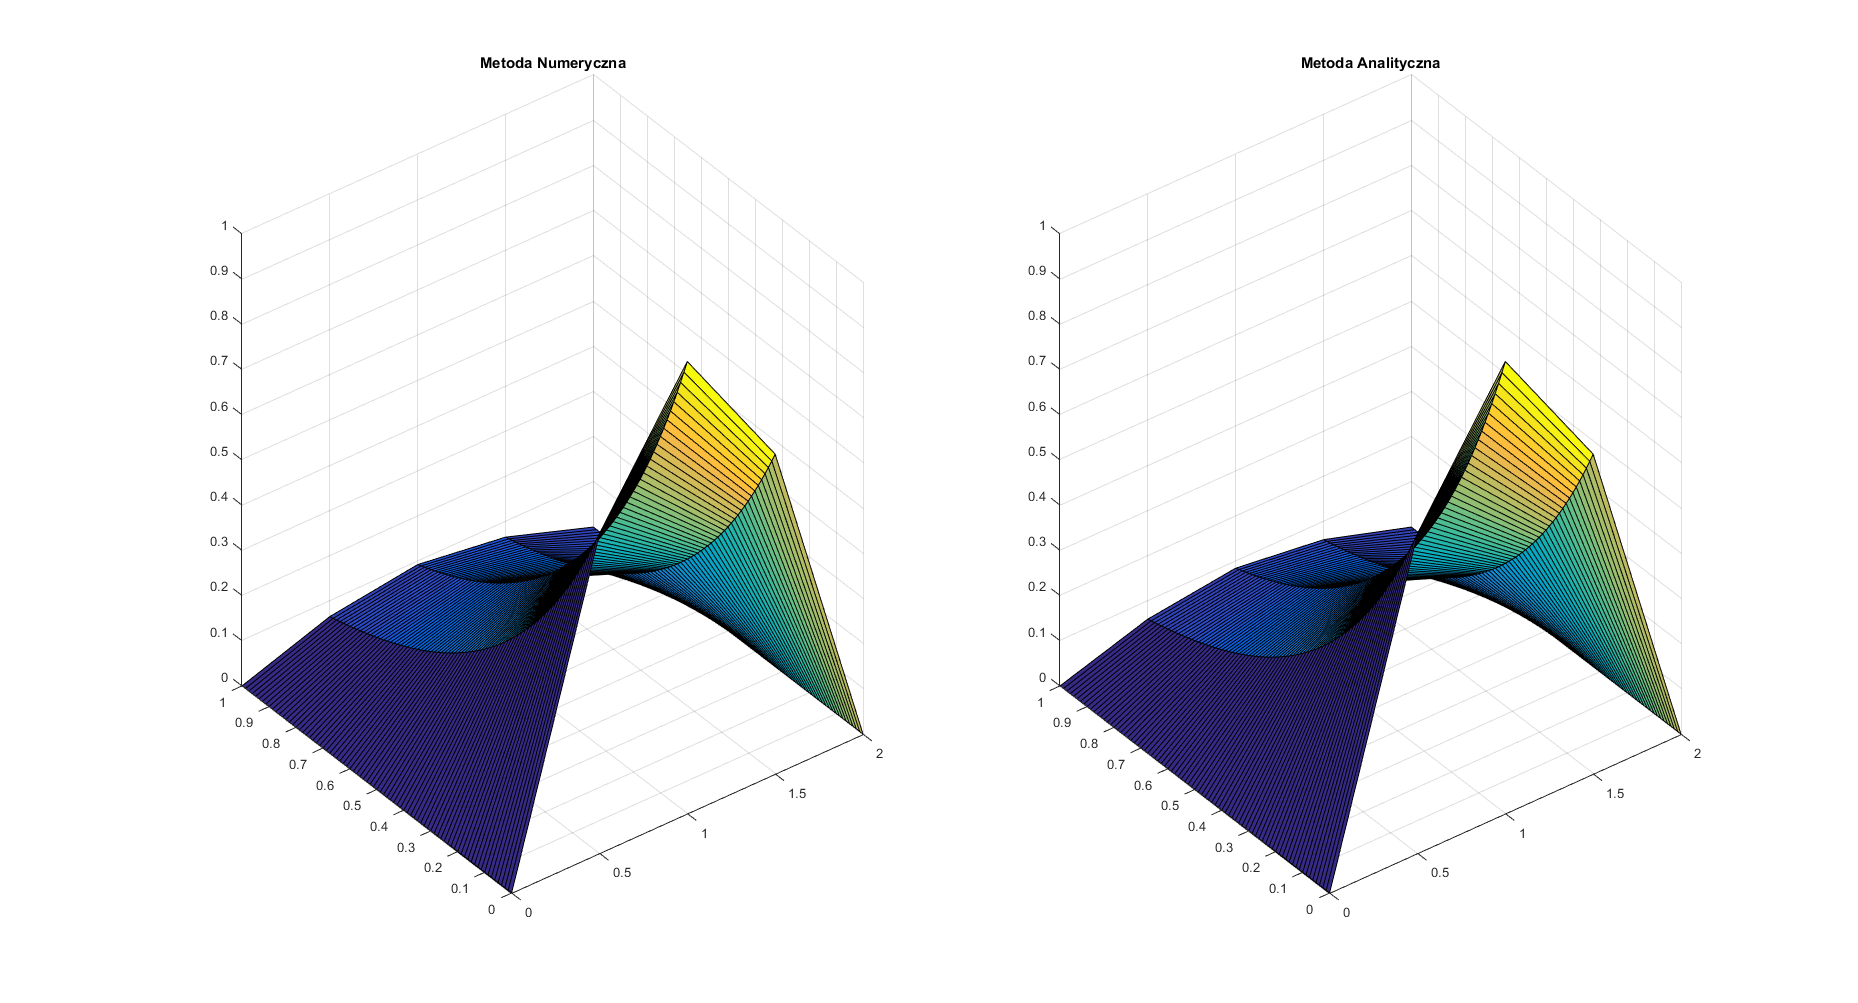
\includegraphics[width=0.78\textwidth]{Lab7/charts/ftcs/5.png}
	\end{center}
\end{figure}

Liczba wykonanych iteracji $ = 80 $

Czas wykonywania algorytmu $ = 0.102 s$

Dla n = 15:

\begin{figure}[!ht]
	\begin{center}
		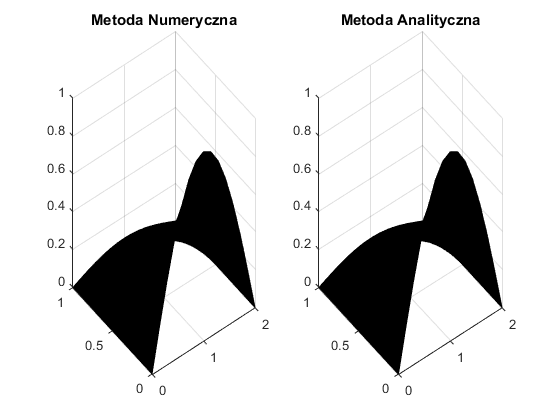
\includegraphics[width=0.78\textwidth]{Lab7/charts/ftcs/15.png}
	\end{center}
\end{figure}

Liczba wykonanych iteracji $ = 405 $

Czas wykonywania algorytmu $ = 0.163 s$

\newpage

Dla n = 30:

\begin{figure}[!ht]
	\begin{center}
		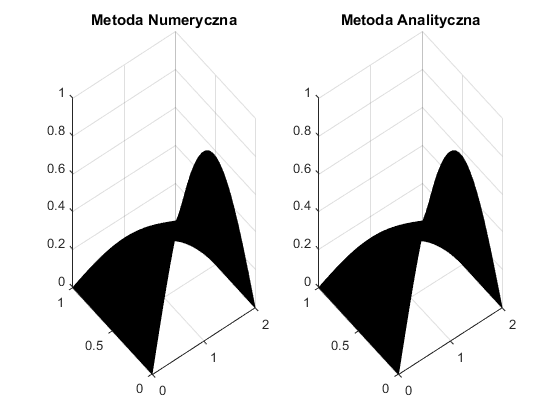
\includegraphics[width=0.78\textwidth]{Lab7/charts/ftcs/30.png}
	\end{center}
\end{figure}

Liczba wykonanych iteracji $ = 4205 $

Czas wykonywania algorytmu $ = 0.472 s$
\newpage
\subsection{Schemat BTCS}
BTCS (ang. Backward Time Central Space) czyli schemat "w tył":

$$\dfrac{\delta \psi}{\delta t} = D\dfrac{\delta^2 \psi}{\delta x^2}$$

Dla lewej strony równania zastosujemy schemat "w tył", natomiast dla prawej schemat centralny.

Mamy więc:

$$\dfrac{\psi^{(n+1)}_{i}-\psi^n_{i}}{\Delta t}=D\dfrac{\psi^{n}_{i+1}-2\psi^n_{i}+\psi^n_{i-1}}{\Delta x^2}$$

Stąd:

$$-\psi^{(n+1)}_{i+1} + \left(2+\dfrac{\Delta x^2}{D \Delta t}\right) \psi^{(n+1)}_{i} -\psi^{(n+1)}_{i-1} =\dfrac{\Delta x^2}{D\Delta t}\psi^{n}_{i}$$

Jest to schemat jawny, bezwzględnie stabilny. 

Z powyższego równania otrzymujemy liniowy układ równań algebraicznych, a więc w każdej iteracji czasowej należy rozwiązać pewien układ równań liniowych.
\newpage
\subsubsection{Algorytm}
\begin{Shaded}
\begin{Highlighting}[]
\FunctionTok{clc}\NormalTok{,}\FunctionTok{clear} \FunctionTok{all}\NormalTok{; }\FunctionTok{tic}
\CommentTok{%rozwiązanie analityczne}
\NormalTok{G = @(x,t) }\FunctionTok{sin}\NormalTok{(}\BaseNTok{pi}\NormalTok{.*x./}\FloatTok{2}\NormalTok{).*}\FunctionTok{exp}\NormalTok{(-(}\BaseNTok{pi}\NormalTok{.^}\FloatTok{2}\NormalTok{).*t./}\FloatTok{4}\NormalTok{);}
\CommentTok{%przedział omega}
\NormalTok{xa=}\FloatTok{0}\NormalTok{; xb=}\FloatTok{2}\NormalTok{; yc=}\FloatTok{0}\NormalTok{; yd=}\FloatTok{1}\NormalTok{;}
\CommentTok{%warunki brzegowe}
\NormalTok{u1 = @(x) }\FloatTok{0}\NormalTok{;}
\NormalTok{u2 = @(x) }\FloatTok{0}\NormalTok{;}
\NormalTok{u3 = @(x,t) }\FunctionTok{sin}\NormalTok{(}\BaseNTok{pi}\NormalTok{*x/}\FloatTok{2}\NormalTok{);}
\NormalTok{licznik=}\FloatTok{0}\NormalTok{;}
\CommentTok{%siatka}
\NormalTok{m=}\FloatTok{20}\NormalTok{; D=}\FloatTok{1}\NormalTok{;}
\NormalTok{deltax=(xb-xa)/(m-}\FloatTok{1}\NormalTok{);}
\NormalTok{x=[xa:deltax:xb];         }\CommentTok{%przedział przestrzenny}
\NormalTok{deltat=(deltax^}\FloatTok{2}\NormalTok{)/(}\FloatTok{10}\NormalTok{*D); }
\NormalTok{n_end=}\FunctionTok{floor}\NormalTok{(yd/deltat)+}\FloatTok{1}\NormalTok{; }
\NormalTok{t=[}\FloatTok{0}\NormalTok{:deltat:}\FloatTok{1}\NormalTok{];           }\CommentTok{%przedział czasowy}
\CommentTok{%macierz}
\FunctionTok{psi}\NormalTok{=}\FunctionTok{zeros}\NormalTok{(n_end,}\FunctionTok{length}\NormalTok{(x)); }\CommentTok{%utworzenie pustej macierzy}
\CommentTok{%dodanie warunku początkowego}
\FunctionTok{psi}\NormalTok{(}\FloatTok{1}\NormalTok{,:) = u3(x);}
\FunctionTok{psi}\NormalTok{(:,}\FloatTok{1}\NormalTok{) = u1(t);}
\FunctionTok{psi}\NormalTok{(:,m) = u2(t);}
\NormalTok{A = (}\FloatTok{2}\NormalTok{+(deltax^}\FloatTok{2}\NormalTok{)/(deltat))*}\FunctionTok{diag}\NormalTok{(}\FunctionTok{eye}\NormalTok{(m-}\FloatTok{2}\NormalTok{));}
\NormalTok{B = }\FunctionTok{diag}\NormalTok{(A) + -}\FloatTok{1}\NormalTok{*}\FunctionTok{diag}\NormalTok{(}\FunctionTok{diag}\NormalTok{(}\FunctionTok{eye}\NormalTok{(m-}\FloatTok{3}\NormalTok{)),-}\FloatTok{1}\NormalTok{) + -}\FloatTok{1}\NormalTok{*}\FunctionTok{diag}\NormalTok{(}\FunctionTok{diag}\NormalTok{(}\FunctionTok{eye}\NormalTok{(m-}\FloatTok{3}\NormalTok{)),}\FloatTok{1}\NormalTok{);}
\NormalTok{for n=}\FloatTok{2}\NormalTok{:n_end}
\NormalTok{  F = }\FunctionTok{diag}\NormalTok{(}\FunctionTok{eye}\NormalTok{(m-}\FloatTok{2}\NormalTok{)) * deltax^}\FloatTok{2}\NormalTok{/deltat .* }\FunctionTok{psi}\NormalTok{(n-}\FloatTok{1}\NormalTok{,}\FloatTok{2}\NormalTok{:m-}\FloatTok{1}\NormalTok{)';}
\NormalTok{  F(}\FloatTok{1}\NormalTok{) = F(}\FloatTok{1}\NormalTok{) + }\FunctionTok{psi}\NormalTok{(n,}\FloatTok{1}\NormalTok{);}
\NormalTok{  F(}\FunctionTok{length}\NormalTok{(F)) = F(}\FunctionTok{length}\NormalTok{(F)) + }\FunctionTok{psi}\NormalTok{(n, m);  }
  \FunctionTok{psi}\NormalTok{(n,}\FloatTok{2}\NormalTok{:m-}\FloatTok{1}\NormalTok{) = linsolve(B,F);}
\NormalTok{  licznik = licznik+}\FloatTok{1}\NormalTok{;}
\NormalTok{end}
\NormalTok{[X,T] = }\FunctionTok{meshgrid}\NormalTok{(x,t);}
\FunctionTok{subplot}\NormalTok{(}\FloatTok{1}\NormalTok{,}\FloatTok{2}\NormalTok{,}\FloatTok{1}\NormalTok{)}
\FunctionTok{surf}\NormalTok{(X,T,}\FunctionTok{psi}\NormalTok{)}
\FunctionTok{title}\NormalTok{(}\StringTok{'Metoda Numeryczna'}\NormalTok{)}
\FunctionTok{subplot}\NormalTok{(}\FloatTok{1}\NormalTok{,}\FloatTok{2}\NormalTok{,}\FloatTok{2}\NormalTok{)}
\FunctionTok{surf}\NormalTok{(X,T,(G(X,T)))}
\FunctionTok{title}\NormalTok{(}\StringTok{'Metoda Analityczna'}\NormalTok{)}
\NormalTok{Error=}\FunctionTok{max}\NormalTok{(}\FunctionTok{max}\NormalTok{(}\FunctionTok{abs}\NormalTok{(}\FunctionTok{psi}\NormalTok{-G(X,T))));}
\NormalTok{licznik; }\FunctionTok{toc}
\end{Highlighting}
\end{Shaded}
\newpage
\subsubsection{Wykresy}

Dla n = 5:

\begin{figure}[!ht]
	\begin{center}
		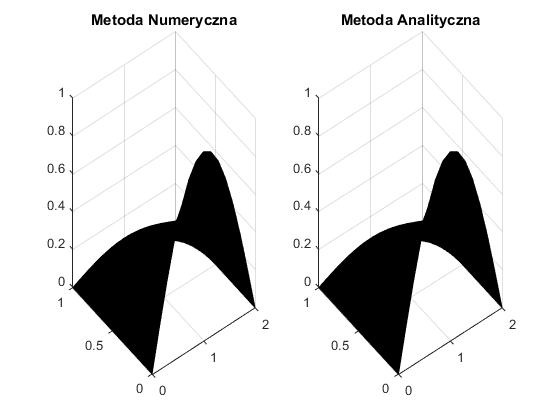
\includegraphics[width=0.78\textwidth]{Lab7/charts/btcs/5.png}
	\end{center}
\end{figure}

Liczba wykonanych iteracji $ = 80 $

Czas wykonywania algorytmu $ = 0.105 s$

Dla n = 15:

\begin{figure}[!ht]
	\begin{center}
		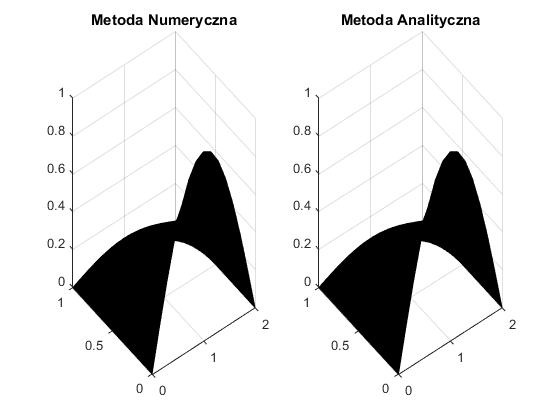
\includegraphics[width=0.78\textwidth]{Lab7/charts/btcs/15.png}
	\end{center}
\end{figure}

Liczba wykonanych iteracji $ = 980 $

Czas wykonywania algorytmu $ = 0.131 s$

\newpage

Dla n = 30:

\begin{figure}[!ht]
	\begin{center}
		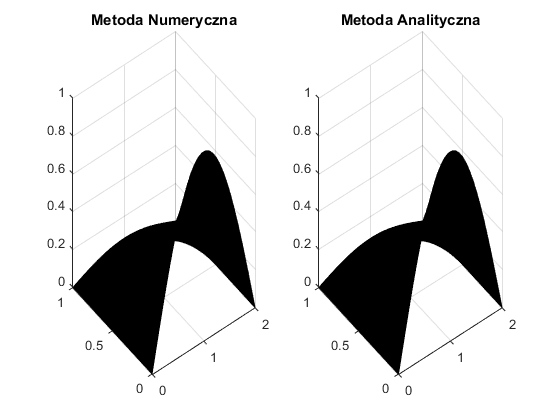
\includegraphics[width=0.78\textwidth]{Lab7/charts/btcs/30.png}
	\end{center}
\end{figure}

Liczba wykonanych iteracji $ = 4205 $

Czas wykonywania algorytmu $ = 0.254 s$
\newpage

\newpage
\subsection{Schemat Cranka-Nicolson}
%TODO
\newpage
\subsubsection{Algorytm}
%\input{Lab7/ctcs}
\newpage
\subsubsection{Wykresy}
\newpage
\subsection{Schemat DuForta-Frankle}
Schemat DuForta-Frankle dla równań dyfuzyjnych postaci:

$$\dfrac{\delta \psi}{\delta t} = D\dfrac{\delta^2 \psi}{\delta x^2}$$

Dla obu stron powyższego równania stosuje się schemat centralny.

Mamy więc:

$$\dfrac{\psi^{(n+1)}_{i}-\psi^{n-1}_{i}}{2\Delta t}=D\dfrac{\psi^{n}_{i+1}- \left( \psi^{(n+1)}_{i} + \psi^{(n-1)}_{i} \right)+\psi^n_{i-1}}{\Delta x^2}$$

Stąd:

$$\psi^{(n+1)}_{i} \left(\dfrac{1}{2 \Delta t} + \dfrac{D}{\Delta x^2}\right)= \dfrac{D}{\Delta x^2} \left( \psi^{n}_{i+1} + \psi^{n}_{i-1} \right) - \psi^{(n-1)}_{i} \left( \dfrac{D}{\Delta x^2} + \dfrac{1}{2\Delta t} \right) $$

Jest to schemat jawny, bezwzględnie stabilny. 

Wadą tej metody jest powstawanie oscylacyjnych rozwiązań dla dużych kroków czasowych, co wpływa na jakość rozwiązania.

Jest to schemat trójpoziomowy, a więc przedstawimy dwa sposoby rozwiązania tego problemu:
\begin{itemize}
	\item skopiujemy warunek początkowy na dwa poziomy
	\item I poziom nieznany zbudujemy za pomocą schematu dwupoziomowego
\end{itemize}

\newpage
\subsubsection{Algorytm}
a)
\begin{Shaded}
\begin{Highlighting}[]
\FunctionTok{clc}\NormalTok{,}\FunctionTok{clear} \FunctionTok{all}
\FunctionTok{tic}
\CommentTok{%rozwiązanie analityczne}
\NormalTok{G = @(x,t) }\FunctionTok{sin}\NormalTok{(}\BaseNTok{pi}\NormalTok{.*x./}\FloatTok{2}\NormalTok{).*}\FunctionTok{exp}\NormalTok{(-(}\BaseNTok{pi}\NormalTok{.^}\FloatTok{2}\NormalTok{).*t./}\FloatTok{4}\NormalTok{);}
\CommentTok{%przedział omega}
\NormalTok{xa=}\FloatTok{0}\NormalTok{; xb=}\FloatTok{2}\NormalTok{; yc=}\FloatTok{0}\NormalTok{; yd=}\FloatTok{1}\NormalTok{;}
\CommentTok{%warunki brzegowe}
\NormalTok{u1 = @(x) }\FloatTok{0}\NormalTok{;}
\NormalTok{u2 = @(x) }\FloatTok{0}\NormalTok{;}
\NormalTok{u3 = @(x,t) }\FunctionTok{sin}\NormalTok{(}\BaseNTok{pi}\NormalTok{*x/}\FloatTok{2}\NormalTok{);}
\NormalTok{licznik=}\FloatTok{0}\NormalTok{;}
\CommentTok{%siatka}
\NormalTok{m=}\FloatTok{40}\NormalTok{; D=}\FloatTok{1}\NormalTok{;}
\NormalTok{deltax=(xb-xa)/(m-}\FloatTok{1}\NormalTok{);}
\NormalTok{x=[xa:deltax:xb];         }\CommentTok{%przedział przestrzenny}
\NormalTok{deltat=(deltax^}\FloatTok{2}\NormalTok{)/(}\FloatTok{10}\NormalTok{*D); }
\NormalTok{n_end=}\FunctionTok{floor}\NormalTok{(yd/deltat)+}\FloatTok{1}\NormalTok{;}
\NormalTok{t=[}\FloatTok{0}\NormalTok{:deltat:}\FloatTok{1}\NormalTok{];           }\CommentTok{%przedział czasowy}
\CommentTok{%macierz}
\FunctionTok{psi}\NormalTok{=}\FunctionTok{zeros}\NormalTok{(n_end,}\FunctionTok{length}\NormalTok{(x)); }\CommentTok{%utworzenie pustej macierzy}
\CommentTok{%dodanie warunku początkowego}
\FunctionTok{psi}\NormalTok{(}\FloatTok{1}\NormalTok{,:) = u3(x);}
\FunctionTok{psi}\NormalTok{(:,}\FloatTok{1}\NormalTok{) = u1(t);}
\FunctionTok{psi}\NormalTok{(:,m) = u2(t);}
\FunctionTok{psi}\NormalTok{(}\FloatTok{2}\NormalTok{,:) = }\FunctionTok{psi}\NormalTok{(}\FloatTok{1}\NormalTok{,:);}
\NormalTok{F = }\FunctionTok{diag}\NormalTok{(}\FunctionTok{eye}\NormalTok{(}\FloatTok{2}\NormalTok{*m-}\FloatTok{2}\NormalTok{));}
\NormalTok{A1 = }\FunctionTok{eye}\NormalTok{(m-}\FloatTok{2}\NormalTok{) .* -(D/deltax^}\FloatTok{2}\NormalTok{-}\FloatTok{1}\NormalTok{/(}\FloatTok{2}\NormalTok{*deltat));}
\NormalTok{A2 = (}\FunctionTok{eye}\NormalTok{(m-}\FloatTok{2}\NormalTok{,m) + }\FunctionTok{diag}\NormalTok{(}\FunctionTok{diag}\NormalTok{(}\FunctionTok{eye}\NormalTok{(m-}\FloatTok{2}\NormalTok{)),}\FloatTok{2}\NormalTok{)(}\FloatTok{1}\NormalTok{:m-}\FloatTok{2}\NormalTok{,:)) .* D/deltax^}\FloatTok{2}\NormalTok{;}
\NormalTok{A = [A1, A2] ./ (}\FloatTok{1}\NormalTok{/(}\FloatTok{2}\NormalTok{*deltat) + D/deltax^}\FloatTok{2}\NormalTok{);}
\NormalTok{for n=}\FloatTok{3}\NormalTok{:n_end}
\NormalTok{  F(}\FloatTok{1}\NormalTok{:m-}\FloatTok{2}\NormalTok{) = }\FunctionTok{psi}\NormalTok{(n-}\FloatTok{2}\NormalTok{,}\FloatTok{2}\NormalTok{:m-}\FloatTok{1}\NormalTok{);}
\NormalTok{  F(m-}\FloatTok{1}\NormalTok{:}\FunctionTok{length}\NormalTok{(F)) = }\FunctionTok{psi}\NormalTok{(n-}\FloatTok{1}\NormalTok{,:);}
  \FunctionTok{psi}\NormalTok{(n,}\FloatTok{2}\NormalTok{:m-}\FloatTok{1}\NormalTok{) = A * F;}
\NormalTok{  licznik = licznik+}\FloatTok{1}\NormalTok{;}
\NormalTok{end}
\NormalTok{[X,T] = }\FunctionTok{meshgrid}\NormalTok{(x,t);}
\FunctionTok{subplot}\NormalTok{(}\FloatTok{1}\NormalTok{,}\FloatTok{2}\NormalTok{,}\FloatTok{1}\NormalTok{)}
\FunctionTok{surf}\NormalTok{(X,T,}\FunctionTok{psi}\NormalTok{)}
\FunctionTok{title}\NormalTok{(}\StringTok{'Metoda Numeryczna'}\NormalTok{)}
\FunctionTok{subplot}\NormalTok{(}\FloatTok{1}\NormalTok{,}\FloatTok{2}\NormalTok{,}\FloatTok{2}\NormalTok{)}
\FunctionTok{surf}\NormalTok{(X,T,(G(X,T)))}
\FunctionTok{title}\NormalTok{(}\StringTok{'Metoda Analityczna'}\NormalTok{)}
\NormalTok{Error=}\FunctionTok{max}\NormalTok{(}\FunctionTok{max}\NormalTok{(}\FunctionTok{abs}\NormalTok{(}\FunctionTok{psi}\NormalTok{-G(X,T))));}
\NormalTok{licznik; }\FunctionTok{toc}
\end{Highlighting}
\end{Shaded}
\newpage
b)
%\begin{Shaded}
\begin{Highlighting}[]
\FunctionTok{clc}\NormalTok{,}\FunctionTok{clear} \FunctionTok{all}
\FunctionTok{tic}
\CommentTok{%rozwiązanie analityczne}
\NormalTok{G = @(x,t) }\FunctionTok{sin}\NormalTok{(}\BaseNTok{pi}\NormalTok{.*x./}\FloatTok{2}\NormalTok{).*}\FunctionTok{exp}\NormalTok{(-(}\BaseNTok{pi}\NormalTok{.^}\FloatTok{2}\NormalTok{).*t./}\FloatTok{4}\NormalTok{);}
\CommentTok{%przedział omega}
\NormalTok{xa=}\FloatTok{0}\NormalTok{; xb=}\FloatTok{2}\NormalTok{; yc=}\FloatTok{0}\NormalTok{; yd=}\FloatTok{1}\NormalTok{;}
\CommentTok{%warunki brzegowe}
\NormalTok{u1 = @(x) }\FloatTok{0}\NormalTok{;}
\NormalTok{u2 = @(x) }\FloatTok{0}\NormalTok{;}
\NormalTok{u3 = @(x,t) }\FunctionTok{sin}\NormalTok{(}\BaseNTok{pi}\NormalTok{*x/}\FloatTok{2}\NormalTok{);}
\NormalTok{licznik=}\FloatTok{0}\NormalTok{;}
\CommentTok{%siatka}
\NormalTok{m=}\FloatTok{40}\NormalTok{; D=}\FloatTok{1}\NormalTok{;}
\NormalTok{deltax=(xb-xa)/(m-}\FloatTok{1}\NormalTok{);}
\NormalTok{x=[xa:deltax:xb];         }\CommentTok{%przedział przestrzenny}
\NormalTok{deltat=(deltax^}\FloatTok{2}\NormalTok{)/(}\FloatTok{10}\NormalTok{*D); }
\NormalTok{n_end=}\FunctionTok{floor}\NormalTok{(yd/deltat)+}\FloatTok{1}\NormalTok{;}
\NormalTok{t=[}\FloatTok{0}\NormalTok{:deltat:}\FloatTok{1}\NormalTok{];           }\CommentTok{%przedział czasowy}
\CommentTok{%macierz}
\FunctionTok{psi}\NormalTok{=}\FunctionTok{zeros}\NormalTok{(n_end,}\FunctionTok{length}\NormalTok{(x)); }\CommentTok{%utworzenie pustej macierzy}
\CommentTok{%dodanie warunku początkowego}
\FunctionTok{psi}\NormalTok{(}\FloatTok{1}\NormalTok{,:) = u3(x);}
\FunctionTok{psi}\NormalTok{(:,}\FloatTok{1}\NormalTok{) = u1(t);}
\FunctionTok{psi}\NormalTok{(:,m) = u2(t);}
\CommentTok{% Pierwszy poziom za pomocą schematu dwupoziomowego}
\NormalTok{A_2 = (}\FloatTok{2}\NormalTok{+(deltax^}\FloatTok{2}\NormalTok{)/(deltat))*}\FunctionTok{diag}\NormalTok{(}\FunctionTok{eye}\NormalTok{(m-}\FloatTok{2}\NormalTok{));}
\NormalTok{B_2 = }\FunctionTok{diag}\NormalTok{(A_2) + -}\FloatTok{1}\NormalTok{*}\FunctionTok{diag}\NormalTok{(}\FunctionTok{diag}\NormalTok{(}\FunctionTok{eye}\NormalTok{(m-}\FloatTok{3}\NormalTok{)),-}\FloatTok{1}\NormalTok{) + -}\FloatTok{1}\NormalTok{*}\FunctionTok{diag}\NormalTok{(}\FunctionTok{diag}\NormalTok{(}\FunctionTok{eye}\NormalTok{(m-}\FloatTok{3}\NormalTok{)),}\FloatTok{1}\NormalTok{);}
\NormalTok{F = }\FunctionTok{diag}\NormalTok{(}\FunctionTok{eye}\NormalTok{(m-}\FloatTok{2}\NormalTok{)) * deltax^}\FloatTok{2}\NormalTok{/deltat .* }\FunctionTok{psi}\NormalTok{(}\FloatTok{1}\NormalTok{,}\FloatTok{2}\NormalTok{:m-}\FloatTok{1}\NormalTok{)';}
\NormalTok{F(}\FloatTok{1}\NormalTok{) = F(}\FloatTok{1}\NormalTok{) + }\FunctionTok{psi}\NormalTok{(}\FloatTok{2}\NormalTok{,}\FloatTok{1}\NormalTok{);}
\NormalTok{F(}\FunctionTok{length}\NormalTok{(F)) = F(}\FunctionTok{length}\NormalTok{(F)) + }\FunctionTok{psi}\NormalTok{(}\FloatTok{2}\NormalTok{, m);  }
\FunctionTok{psi}\NormalTok{(}\FloatTok{2}\NormalTok{,}\FloatTok{2}\NormalTok{:m-}\FloatTok{1}\NormalTok{) = linsolve(B_2,F);}
\CommentTok{% Pozostałe poziomy}
\NormalTok{F = }\FunctionTok{diag}\NormalTok{(}\FunctionTok{eye}\NormalTok{(}\FloatTok{2}\NormalTok{*m-}\FloatTok{2}\NormalTok{));}
\NormalTok{A1 = }\FunctionTok{eye}\NormalTok{(m-}\FloatTok{2}\NormalTok{) .* -(D/deltax^}\FloatTok{2}\NormalTok{-}\FloatTok{1}\NormalTok{/(}\FloatTok{2}\NormalTok{*deltat));}
\NormalTok{A2 = (}\FunctionTok{eye}\NormalTok{(m-}\FloatTok{2}\NormalTok{,m) + }\FunctionTok{diag}\NormalTok{(}\FunctionTok{diag}\NormalTok{(}\FunctionTok{eye}\NormalTok{(m-}\FloatTok{2}\NormalTok{)),}\FloatTok{2}\NormalTok{)(}\FloatTok{1}\NormalTok{:m-}\FloatTok{2}\NormalTok{,:)) .* D/deltax^}\FloatTok{2}\NormalTok{;}
\NormalTok{A = [A1, A2] ./ (}\FloatTok{1}\NormalTok{/(}\FloatTok{2}\NormalTok{*deltat) + D/deltax^}\FloatTok{2}\NormalTok{);}
\NormalTok{for n=}\FloatTok{3}\NormalTok{:n_end}
\NormalTok{  F(}\FloatTok{1}\NormalTok{:m-}\FloatTok{2}\NormalTok{) = }\FunctionTok{psi}\NormalTok{(n-}\FloatTok{2}\NormalTok{,}\FloatTok{2}\NormalTok{:m-}\FloatTok{1}\NormalTok{);}
\NormalTok{  F(m-}\FloatTok{1}\NormalTok{:}\FunctionTok{length}\NormalTok{(F)) = }\FunctionTok{psi}\NormalTok{(n-}\FloatTok{1}\NormalTok{,:);}
  \FunctionTok{psi}\NormalTok{(n,}\FloatTok{2}\NormalTok{:m-}\FloatTok{1}\NormalTok{) = A * F;}
\NormalTok{  licznik = licznik+}\FloatTok{1}\NormalTok{;}
\NormalTok{end}
\NormalTok{[X,T] = }\FunctionTok{meshgrid}\NormalTok{(x,t);}
\FunctionTok{subplot}\NormalTok{(}\FloatTok{1}\NormalTok{,}\FloatTok{2}\NormalTok{,}\FloatTok{1}\NormalTok{)}
\FunctionTok{surf}\NormalTok{(X,T,}\FunctionTok{psi}\NormalTok{)}
\FunctionTok{title}\NormalTok{(}\StringTok{'Metoda Numeryczna'}\NormalTok{)}
\FunctionTok{subplot}\NormalTok{(}\FloatTok{1}\NormalTok{,}\FloatTok{2}\NormalTok{,}\FloatTok{2}\NormalTok{)}
\FunctionTok{surf}\NormalTok{(X,T,(G(X,T)))}
\FunctionTok{title}\NormalTok{(}\StringTok{'Metoda Analityczna'}\NormalTok{)}
\NormalTok{Error=}\FunctionTok{max}\NormalTok{(}\FunctionTok{max}\NormalTok{(}\FunctionTok{abs}\NormalTok{(}\FunctionTok{psi}\NormalTok{-G(X,T))));}
\NormalTok{licznik; }\FunctionTok{toc}
\end{Highlighting}
\end{Shaded}
\newpage
\subsubsection{Wykresy}
\newpage
\subsection{Schemat Richtmyera-Morton}
\newpage
\subsubsection{Algorytm}
a)
\begin{Shaded}
\begin{Highlighting}[]
\FunctionTok{clc}\NormalTok{,}\FunctionTok{clear} \FunctionTok{all}\NormalTok{; }\FunctionTok{tic}
\CommentTok{%rozwiązanie analityczne}
\NormalTok{G = @(x,t) }\FunctionTok{sin}\NormalTok{(}\BaseNTok{pi}\NormalTok{.*x./}\FloatTok{2}\NormalTok{).*}\FunctionTok{exp}\NormalTok{(-(}\BaseNTok{pi}\NormalTok{.^}\FloatTok{2}\NormalTok{).*t./}\FloatTok{4}\NormalTok{);}
\CommentTok{%przedział omega}
\NormalTok{xa=}\FloatTok{0}\NormalTok{; xb=}\FloatTok{2}\NormalTok{; yc=}\FloatTok{0}\NormalTok{; yd=}\FloatTok{1}\NormalTok{;}
\CommentTok{%warunki brzegowe}
\NormalTok{u1 = @(x) }\FloatTok{0}\NormalTok{;}
\NormalTok{u2 = @(x) }\FloatTok{0}\NormalTok{;}
\NormalTok{u3 = @(x,t) }\FunctionTok{sin}\NormalTok{(}\BaseNTok{pi}\NormalTok{*x/}\FloatTok{2}\NormalTok{);}
\NormalTok{licznik=}\FloatTok{0}\NormalTok{;}
\CommentTok{%siatka}
\NormalTok{m=}\FloatTok{50}\NormalTok{; D=}\FloatTok{1}\NormalTok{;}
\NormalTok{deltax=(xb-xa)/(m-}\FloatTok{1}\NormalTok{);}
\NormalTok{x=[xa:deltax:xb];         }\CommentTok{%przedział przestrzenny}
\NormalTok{deltat=(deltax^}\FloatTok{2}\NormalTok{)/D; n_end=}\FunctionTok{floor}\NormalTok{(yd/deltat)+}\FloatTok{1}\NormalTok{;}
\NormalTok{t=[}\FloatTok{0}\NormalTok{:deltat:}\FloatTok{1}\NormalTok{];           }\CommentTok{%przedział czasowy}
\NormalTok{theta = }\FloatTok{1}\NormalTok{/}\FloatTok{2}\NormalTok{ - deltax^}\FloatTok{2}\NormalTok{ / (}\FloatTok{12}\NormalTok{ * D * deltat);}
\NormalTok{alfa = D * deltat / deltax^}\FloatTok{2}\NormalTok{;}
\CommentTok{%macierz}
\FunctionTok{psi}\NormalTok{=}\FunctionTok{zeros}\NormalTok{(n_end,}\FunctionTok{length}\NormalTok{(x)); }\CommentTok{%utworzenie pustej macierzy}
\CommentTok{%dodanie warunku początkowego}
\FunctionTok{psi}\NormalTok{(}\FloatTok{1}\NormalTok{,:) = u3(x);}
\FunctionTok{psi}\NormalTok{(:,}\FloatTok{1}\NormalTok{) = u1(t);}
\FunctionTok{psi}\NormalTok{(:,m) = u2(t);}
\CommentTok{% Skopiowanie pierwszego kroku }
\FunctionTok{psi}\NormalTok{(}\FloatTok{2}\NormalTok{,:) = }\FunctionTok{psi}\NormalTok{(}\FloatTok{1}\NormalTok{,:);}
\NormalTok{F = }\FunctionTok{diag}\NormalTok{(}\FunctionTok{eye}\NormalTok{(m-}\FloatTok{2}\NormalTok{));}
\NormalTok{A1 = }\FunctionTok{eye}\NormalTok{(m-}\FloatTok{2}\NormalTok{) .* (}\FloatTok{2}\NormalTok{*alfa + }\FloatTok{1}\NormalTok{ + theta);}
\NormalTok{A2 = }\FunctionTok{diag}\NormalTok{(}\FunctionTok{eye}\NormalTok{(m-}\FloatTok{3}\NormalTok{)) * -alfa;}
\NormalTok{A = A1 + }\FunctionTok{diag}\NormalTok{(A2,-}\FloatTok{1}\NormalTok{) + }\FunctionTok{diag}\NormalTok{(A2, }\FloatTok{1}\NormalTok{);}
\NormalTok{for n=}\FloatTok{3}\NormalTok{:n_end}
\NormalTok{  F = (}\FloatTok{1}\NormalTok{+}\FloatTok{2}\NormalTok{*theta) * }\FunctionTok{psi}\NormalTok{(n-}\FloatTok{1}\NormalTok{,}\FloatTok{2}\NormalTok{:m-}\FloatTok{1}\NormalTok{) - theta * }\FunctionTok{psi}\NormalTok{(n-}\FloatTok{2}\NormalTok{, }\FloatTok{2}\NormalTok{:m-}\FloatTok{1}\NormalTok{);}
\NormalTok{  F(}\FloatTok{1}\NormalTok{) = F(}\FloatTok{1}\NormalTok{) + alfa * }\FunctionTok{psi}\NormalTok{(n, }\FloatTok{1}\NormalTok{);}
\NormalTok{  F(m-}\FloatTok{2}\NormalTok{) = F(m-}\FloatTok{2}\NormalTok{) + alfa * }\FunctionTok{psi}\NormalTok{(n, m);}
  \FunctionTok{psi}\NormalTok{(n,}\FloatTok{2}\NormalTok{:m-}\FloatTok{1}\NormalTok{) = linsolve(A,F');}
\NormalTok{  licznik = licznik+}\FloatTok{1}\NormalTok{;}
\NormalTok{end}
\NormalTok{[X,T] = }\FunctionTok{meshgrid}\NormalTok{(x,t);}
\FunctionTok{subplot}\NormalTok{(}\FloatTok{1}\NormalTok{,}\FloatTok{2}\NormalTok{,}\FloatTok{1}\NormalTok{)}
\FunctionTok{surf}\NormalTok{(X,T,}\FunctionTok{psi}\NormalTok{)}
\FunctionTok{title}\NormalTok{(}\StringTok{'Metoda Numeryczna'}\NormalTok{)}
\FunctionTok{subplot}\NormalTok{(}\FloatTok{1}\NormalTok{,}\FloatTok{2}\NormalTok{,}\FloatTok{2}\NormalTok{)}
\FunctionTok{surf}\NormalTok{(X,T,(G(X,T)))}
\FunctionTok{title}\NormalTok{(}\StringTok{'Metoda Analityczna'}\NormalTok{)}
\NormalTok{Error=}\FunctionTok{max}\NormalTok{(}\FunctionTok{max}\NormalTok{(}\FunctionTok{abs}\NormalTok{(}\FunctionTok{psi}\NormalTok{-G(X,T))));}
\NormalTok{licznik; }\FunctionTok{toc}
\end{Highlighting}
\end{Shaded}
\newpage
b)
\begin{Shaded}
\begin{Highlighting}[]
\FunctionTok{clc}\NormalTok{, }\FunctionTok{clear} \FunctionTok{all}\NormalTok{; }\FunctionTok{tic}
\CommentTok{%rozwiązanie analityczne}
\NormalTok{G = @(x,t) }\FunctionTok{sin}\NormalTok{(}\BaseNTok{pi}\NormalTok{.*x./}\FloatTok{2}\NormalTok{).*}\FunctionTok{exp}\NormalTok{(-(}\BaseNTok{pi}\NormalTok{.^}\FloatTok{2}\NormalTok{).*t./}\FloatTok{4}\NormalTok{);}
\CommentTok{%przedział omega}
\NormalTok{xa=}\FloatTok{0}\NormalTok{; xb=}\FloatTok{2}\NormalTok{; yc=}\FloatTok{0}\NormalTok{; yd=}\FloatTok{1}\NormalTok{;}
\CommentTok{%warunki brzegowe}
\NormalTok{u1 = @(x) }\FloatTok{0}\NormalTok{; u2 = @(x) }\FloatTok{0}\NormalTok{; u3 = @(x,t) }\FunctionTok{sin}\NormalTok{(}\BaseNTok{pi}\NormalTok{*x/}\FloatTok{2}\NormalTok{);}
\NormalTok{licznik=}\FloatTok{0}\NormalTok{;}
\CommentTok{%siatka}
\NormalTok{m=}\FloatTok{50}\NormalTok{; D=}\FloatTok{1}\NormalTok{; deltax=(xb-xa)/(m-}\FloatTok{1}\NormalTok{);}
\NormalTok{x=[xa:deltax:xb];         }\CommentTok{%przedział przestrzenny}
\NormalTok{deltat=(deltax^}\FloatTok{2}\NormalTok{)/D; }
\NormalTok{n_end=}\FunctionTok{floor}\NormalTok{(yd/deltat)+}\FloatTok{1}\NormalTok{;}
\NormalTok{t=[}\FloatTok{0}\NormalTok{:deltat:}\FloatTok{1}\NormalTok{];           }\CommentTok{%przedział czasowy}
\NormalTok{theta = }\FloatTok{1}\NormalTok{/}\FloatTok{2}\NormalTok{ - deltax^}\FloatTok{2}\NormalTok{ / (}\FloatTok{12}\NormalTok{ * D * deltat);}
\NormalTok{alfa = D * deltat / deltax^}\FloatTok{2}\NormalTok{;}
\CommentTok{%macierz}
\FunctionTok{psi}\NormalTok{=}\FunctionTok{zeros}\NormalTok{(n_end,}\FunctionTok{length}\NormalTok{(x)); }\CommentTok{%utworzenie pustej macierzy}
\CommentTok{%dodanie warunku początkowego}
\FunctionTok{psi}\NormalTok{(}\FloatTok{1}\NormalTok{,:) = u3(x);}
\FunctionTok{psi}\NormalTok{(:,}\FloatTok{1}\NormalTok{) = u1(t);}
\FunctionTok{psi}\NormalTok{(:,m) = u2(t);}
\NormalTok{A1 = }\FunctionTok{eye}\NormalTok{(m-}\FloatTok{2}\NormalTok{) .* (}\FloatTok{2}\NormalTok{*alfa + }\FloatTok{1}\NormalTok{ + theta);}
\NormalTok{A2 = }\FunctionTok{diag}\NormalTok{(}\FunctionTok{eye}\NormalTok{(m-}\FloatTok{3}\NormalTok{)) * -alfa;}
\NormalTok{A = A1 + }\FunctionTok{diag}\NormalTok{(A2,-}\FloatTok{1}\NormalTok{) + }\FunctionTok{diag}\NormalTok{(A2, }\FloatTok{1}\NormalTok{);}
\CommentTok{% Pierwszy poziom za pomocą schematu dwupoziomowego}
\NormalTok{A_2 = (}\FloatTok{2}\NormalTok{+(deltax^}\FloatTok{2}\NormalTok{)/(deltat))*}\FunctionTok{diag}\NormalTok{(}\FunctionTok{eye}\NormalTok{(m-}\FloatTok{2}\NormalTok{));}
\NormalTok{B_2 = }\FunctionTok{diag}\NormalTok{(A_2) + -}\FloatTok{1}\NormalTok{*}\FunctionTok{diag}\NormalTok{(}\FunctionTok{diag}\NormalTok{(}\FunctionTok{eye}\NormalTok{(m-}\FloatTok{3}\NormalTok{)),-}\FloatTok{1}\NormalTok{) + -}\FloatTok{1}\NormalTok{*}\FunctionTok{diag}\NormalTok{(}\FunctionTok{diag}\NormalTok{(}\FunctionTok{eye}\NormalTok{(m-}\FloatTok{3}\NormalTok{)),}\FloatTok{1}\NormalTok{);}
\NormalTok{F = }\FunctionTok{diag}\NormalTok{(}\FunctionTok{eye}\NormalTok{(m-}\FloatTok{2}\NormalTok{)) * deltax^}\FloatTok{2}\NormalTok{/deltat .* }\FunctionTok{psi}\NormalTok{(}\FloatTok{1}\NormalTok{,}\FloatTok{2}\NormalTok{:m-}\FloatTok{1}\NormalTok{)';}
\NormalTok{F(}\FloatTok{1}\NormalTok{) = F(}\FloatTok{1}\NormalTok{) + }\FunctionTok{psi}\NormalTok{(}\FloatTok{2}\NormalTok{,}\FloatTok{1}\NormalTok{); F(}\FunctionTok{length}\NormalTok{(F)) = F(}\FunctionTok{length}\NormalTok{(F)) + }\FunctionTok{psi}\NormalTok{(}\FloatTok{2}\NormalTok{, m);  }
\FunctionTok{psi}\NormalTok{(}\FloatTok{2}\NormalTok{,}\FloatTok{2}\NormalTok{:m-}\FloatTok{1}\NormalTok{) = linsolve(B_2,F);}
\CommentTok{% Pozostałe poziomy}
\NormalTok{for n=}\FloatTok{3}\NormalTok{:n_end}
\NormalTok{  F = (}\FloatTok{1}\NormalTok{+}\FloatTok{2}\NormalTok{*theta) * }\FunctionTok{psi}\NormalTok{(n-}\FloatTok{1}\NormalTok{,}\FloatTok{2}\NormalTok{:m-}\FloatTok{1}\NormalTok{) - theta * }\FunctionTok{psi}\NormalTok{(n-}\FloatTok{2}\NormalTok{, }\FloatTok{2}\NormalTok{:m-}\FloatTok{1}\NormalTok{);}
\NormalTok{  F(}\FloatTok{1}\NormalTok{) = F(}\FloatTok{1}\NormalTok{) + alfa * }\FunctionTok{psi}\NormalTok{(n, }\FloatTok{1}\NormalTok{);}
\NormalTok{  F(m-}\FloatTok{2}\NormalTok{) = F(m-}\FloatTok{2}\NormalTok{) + alfa * }\FunctionTok{psi}\NormalTok{(n, m);}
  \FunctionTok{psi}\NormalTok{(n,}\FloatTok{2}\NormalTok{:m-}\FloatTok{1}\NormalTok{) = linsolve(A,F');}
\NormalTok{  licznik = licznik+}\FloatTok{1}\NormalTok{;}
\NormalTok{end}
\NormalTok{[X,T] = }\FunctionTok{meshgrid}\NormalTok{(x,t);}
\FunctionTok{subplot}\NormalTok{(}\FloatTok{1}\NormalTok{,}\FloatTok{2}\NormalTok{,}\FloatTok{1}\NormalTok{)}
\FunctionTok{surf}\NormalTok{(X,T,}\FunctionTok{psi}\NormalTok{)}
\FunctionTok{title}\NormalTok{(}\StringTok{'Metoda Numeryczna'}\NormalTok{)}
\FunctionTok{subplot}\NormalTok{(}\FloatTok{1}\NormalTok{,}\FloatTok{2}\NormalTok{,}\FloatTok{2}\NormalTok{)}
\FunctionTok{surf}\NormalTok{(X,T,(G(X,T)))}
\FunctionTok{title}\NormalTok{(}\StringTok{'Metoda Analityczna'}\NormalTok{)}
\NormalTok{Error=}\FunctionTok{max}\NormalTok{(}\FunctionTok{max}\NormalTok{(}\FunctionTok{abs}\NormalTok{(}\FunctionTok{psi}\NormalTok{-G(X,T))));}
\NormalTok{licznik; }\FunctionTok{toc}
\end{Highlighting}
\end{Shaded}
\newpage
\subsubsection{Wykresy}
\newpage
